\documentclass[1p]{elsarticle_modified}
%\bibliographystyle{elsarticle-num}

%\usepackage[colorlinks]{hyperref}
%\usepackage{abbrmath_seonhwa} %\Abb, \Ascr, \Acal ,\Abf, \Afrak
\usepackage{amsfonts}
\usepackage{amssymb}
\usepackage{amsmath}
\usepackage{amsthm}
\usepackage{scalefnt}
\usepackage{amsbsy}
\usepackage{kotex}
\usepackage{caption}
\usepackage{subfig}
\usepackage{color}
\usepackage{graphicx}
\usepackage{xcolor} %% white, black, red, green, blue, cyan, magenta, yellow
\usepackage{float}
\usepackage{setspace}
\usepackage{hyperref}

\usepackage{tikz}
\usetikzlibrary{arrows}

\usepackage{multirow}
\usepackage{array} % fixed length table
\usepackage{hhline}

%%%%%%%%%%%%%%%%%%%%%
\makeatletter
\renewcommand*\env@matrix[1][\arraystretch]{%
	\edef\arraystretch{#1}%
	\hskip -\arraycolsep
	\let\@ifnextchar\new@ifnextchar
	\array{*\c@MaxMatrixCols c}}
\makeatother %https://tex.stackexchange.com/questions/14071/how-can-i-increase-the-line-spacing-in-a-matrix
%%%%%%%%%%%%%%%

\usepackage[normalem]{ulem}

\newcommand{\msout}[1]{\ifmmode\text{\sout{\ensuremath{#1}}}\else\sout{#1}\fi}
%SOURCE: \msout is \stkout macro in https://tex.stackexchange.com/questions/20609/strikeout-in-math-mode

\newcommand{\cancel}[1]{
	\ifmmode
	{\color{red}\msout{#1}}
	\else
	{\color{red}\sout{#1}}
	\fi
}

\newcommand{\add}[1]{
	{\color{blue}\uwave{#1}}
}

\newcommand{\replace}[2]{
	\ifmmode
	{\color{red}\msout{#1}}{\color{blue}\uwave{#2}}
	\else
	{\color{red}\sout{#1}}{\color{blue}\uwave{#2}}
	\fi
}

\newcommand{\Sol}{\mathcal{S}} %segment
\newcommand{\D}{D} %diagram
\newcommand{\A}{\mathcal{A}} %arc


%%%%%%%%%%%%%%%%%%%%%%%%%%%%%5 test

\def\sl{\operatorname{\textup{SL}}(2,\Cbb)}
\def\psl{\operatorname{\textup{PSL}}(2,\Cbb)}
\def\quan{\mkern 1mu \triangleright \mkern 1mu}

\theoremstyle{definition}
\newtheorem{thm}{Theorem}[section]
\newtheorem{prop}[thm]{Proposition}
\newtheorem{lem}[thm]{Lemma}
\newtheorem{ques}[thm]{Question}
\newtheorem{cor}[thm]{Corollary}
\newtheorem{defn}[thm]{Definition}
\newtheorem{exam}[thm]{Example}
\newtheorem{rmk}[thm]{Remark}
\newtheorem{alg}[thm]{Algorithm}

\newcommand{\I}{\sqrt{-1}}
\begin{document}

%\begin{frontmatter}
%
%\title{Boundary parabolic representations of knots up to 8 crossings}
%
%%% Group authors per affiliation:
%\author{Yunhi Cho} 
%\address{Department of Mathematics, University of Seoul, Seoul, Korea}
%\ead{yhcho@uos.ac.kr}
%
%
%\author{Seonhwa Kim} %\fnref{s_kim}}
%\address{Center for Geometry and Physics, Institute for Basic Science, Pohang, 37673, Korea}
%\ead{ryeona17@ibs.re.kr}
%
%\author{Hyuk Kim}
%\address{Department of Mathematical Sciences, Seoul National University, Seoul 08826, Korea}
%\ead{hyukkim@snu.ac.kr}
%
%\author{Seokbeom Yoon}
%\address{Department of Mathematical Sciences, Seoul National University, Seoul, 08826,  Korea}
%\ead{sbyoon15@snu.ac.kr}
%
%\begin{abstract}
%We find all boundary parabolic representation of knots up to 8 crossings.
%
%\end{abstract}
%\begin{keyword}
%    \MSC[2010] 57M25 
%\end{keyword}
%
%\end{frontmatter}

%\linenumbers
%\tableofcontents
%
\newcommand\colored[1]{\textcolor{white}{\rule[-0.35ex]{0.8em}{1.4ex}}\kern-0.8em\color{red} #1}%
%\newcommand\colored[1]{\textcolor{white}{ #1}\kern-2.17ex	\textcolor{white}{ #1}\kern-1.81ex	\textcolor{white}{ #1}\kern-2.15ex\color{red}#1	}

{\Large $\underline{11a_{165}~(K11a_{165})}$}

\setlength{\tabcolsep}{10pt}
\renewcommand{\arraystretch}{1.6}
\vspace{1cm}\begin{tabular}{m{100pt}>{\centering\arraybackslash}m{274pt}}
\multirow{5}{120pt}{
	\centering
	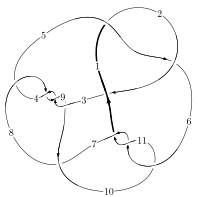
\includegraphics[width=112pt]{../../../GIT/diagram.site/Diagrams/png/414_11a_165.png}\\
\ \ \ A knot diagram\footnotemark}&
\allowdisplaybreaks
\textbf{Linearized knot diagam} \\
\cline{2-2}
 &
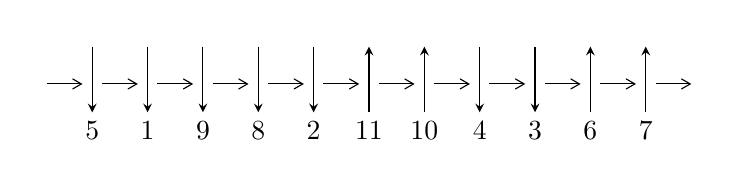
\begin{tikzpicture}[x=20pt, y=17pt]
	% nodes
	\node (C0) at (0, 0) {};
	\node (C1) at (1, 0) {};
	\node (C1U) at (1, +1) {};
	\node (C1D) at (1, -1) {5};

	\node (C2) at (2, 0) {};
	\node (C2U) at (2, +1) {};
	\node (C2D) at (2, -1) {1};

	\node (C3) at (3, 0) {};
	\node (C3U) at (3, +1) {};
	\node (C3D) at (3, -1) {9};

	\node (C4) at (4, 0) {};
	\node (C4U) at (4, +1) {};
	\node (C4D) at (4, -1) {8};

	\node (C5) at (5, 0) {};
	\node (C5U) at (5, +1) {};
	\node (C5D) at (5, -1) {2};

	\node (C6) at (6, 0) {};
	\node (C6U) at (6, +1) {};
	\node (C6D) at (6, -1) {11};

	\node (C7) at (7, 0) {};
	\node (C7U) at (7, +1) {};
	\node (C7D) at (7, -1) {10};

	\node (C8) at (8, 0) {};
	\node (C8U) at (8, +1) {};
	\node (C8D) at (8, -1) {4};

	\node (C9) at (9, 0) {};
	\node (C9U) at (9, +1) {};
	\node (C9D) at (9, -1) {3};

	\node (C10) at (10, 0) {};
	\node (C10U) at (10, +1) {};
	\node (C10D) at (10, -1) {6};

	\node (C11) at (11, 0) {};
	\node (C11U) at (11, +1) {};
	\node (C11D) at (11, -1) {7};
	\node (C12) at (12, 0) {};

	% arrows
	\draw[->,>={angle 60}]
	(C0) edge (C1) (C1) edge (C2) (C2) edge (C3) (C3) edge (C4) (C4) edge (C5) (C5) edge (C6) (C6) edge (C7) (C7) edge (C8) (C8) edge (C9) (C9) edge (C10) (C10) edge (C11) (C11) edge (C12) ;	\draw[->,>=stealth]
	(C1U) edge (C1D) (C2U) edge (C2D) (C3U) edge (C3D) (C4U) edge (C4D) (C5U) edge (C5D) (C6D) edge (C6U) (C7D) edge (C7U) (C8U) edge (C8D) (C9U) edge (C9D) (C10D) edge (C10U) (C11D) edge (C11U) ;
	\end{tikzpicture} \\
\hhline{~~} \\& 
\textbf{Solving Sequence} \\ \cline{2-2} 
 &
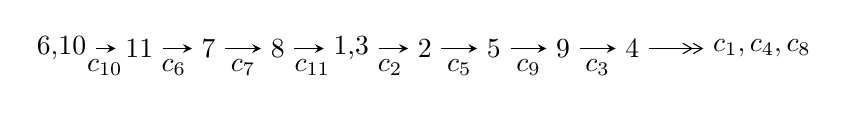
\begin{tikzpicture}[x=25pt, y=7pt]
	% node
	\node (A0) at (-1/8, 0) {6,10};
	\node (A1) at (1, 0) {11};
	\node (A2) at (2, 0) {7};
	\node (A3) at (3, 0) {8};
	\node (A4) at (65/16, 0) {1,3};
	\node (A5) at (41/8, 0) {2};
	\node (A6) at (49/8, 0) {5};
	\node (A7) at (57/8, 0) {9};
	\node (A8) at (65/8, 0) {4};
	\node (C1) at (1/2, -1) {$c_{10}$};
	\node (C2) at (3/2, -1) {$c_{6}$};
	\node (C3) at (5/2, -1) {$c_{7}$};
	\node (C4) at (7/2, -1) {$c_{11}$};
	\node (C5) at (37/8, -1) {$c_{2}$};
	\node (C6) at (45/8, -1) {$c_{5}$};
	\node (C7) at (53/8, -1) {$c_{9}$};
	\node (C8) at (61/8, -1) {$c_{3}$};
	\node (A9) at (10, 0) {$c_{1},c_{4},c_{8}$};

	% edge
	\draw[->,>=stealth]	
	(A0) edge (A1) (A1) edge (A2) (A2) edge (A3) (A3) edge (A4) (A4) edge (A5) (A5) edge (A6) (A6) edge (A7) (A7) edge (A8) ;
	\draw[->>,>={angle 60}]	
	(A8) edge (A9);
\end{tikzpicture} \\ 

\end{tabular} \\

\footnotetext{
The image of knot diagram is generated by the software ``\textbf{Draw programme}" developed by Andrew Bartholomew(\url{http://www.layer8.co.uk/maths/draw/index.htm\#Running-draw}), where we modified some parts for our purpose(\url{https://github.com/CATsTAILs/LinksPainter}).
}\phantom \\ \newline 
\centering \textbf{Ideals for irreducible components\footnotemark of $X_{\text{par}}$} 
 
\begin{align*}
I^u_{1}&=\langle 
-63586 u^{30}-96933 u^{29}+\cdots+270694 b+252865,\\
\phantom{I^u_{1}}&\phantom{= \langle  }-172973 u^{30}+5647 u^{29}+\cdots+406041 a+576964,\;u^{31}-2 u^{30}+\cdots+7 u+3\rangle \\
I^u_{2}&=\langle 
- u^6+2 u^4- u^2+b,\;u^4- u^2+a+1,\;u^{12}-4 u^{10}- u^9+6 u^8+3 u^7-3 u^6-3 u^5- u^4+u^3+u^2+1\rangle \\
I^u_{3}&=\langle 
b^2+2,\;a-1,\;u+1\rangle \\
I^u_{4}&=\langle 
b,\;a-1,\;u-1\rangle \\
\\
\end{align*}
\raggedright * 4 irreducible components of $\dim_{\mathbb{C}}=0$, with total 46 representations.\\
\footnotetext{All coefficients of polynomials are rational numbers. But the coefficients are sometimes approximated in decimal forms when there is not enough margin.}
\newpage
\renewcommand{\arraystretch}{1}
\centering \section*{I. $I^u_{1}= \langle -6.36\times10^{4} u^{30}-9.69\times10^{4} u^{29}+\cdots+2.71\times10^{5} b+2.53\times10^{5},\;-1.73\times10^{5} u^{30}+5647 u^{29}+\cdots+4.06\times10^{5} a+5.77\times10^{5},\;u^{31}-2 u^{30}+\cdots+7 u+3 \rangle$}
\flushleft \textbf{(i) Arc colorings}\\
\begin{tabular}{m{7pt} m{180pt} m{7pt} m{180pt} }
\flushright $a_{6}=$&$\begin{pmatrix}0\\u\end{pmatrix}$ \\
\flushright $a_{10}=$&$\begin{pmatrix}1\\0\end{pmatrix}$ \\
\flushright $a_{11}=$&$\begin{pmatrix}1\\- u^2\end{pmatrix}$ \\
\flushright $a_{7}=$&$\begin{pmatrix}u\\- u^3+u\end{pmatrix}$ \\
\flushright $a_{8}=$&$\begin{pmatrix}- u^3+2 u\\- u^3+u\end{pmatrix}$ \\
\flushright $a_{1}=$&$\begin{pmatrix}- u^2+1\\u^4-2 u^2\end{pmatrix}$ \\
\flushright $a_{3}=$&$\begin{pmatrix}0.425999 u^{30}-0.0139075 u^{29}+\cdots+0.292554 u-1.42095\\0.234900 u^{30}+0.358091 u^{29}+\cdots-0.536610 u-0.934136\end{pmatrix}$ \\
\flushright $a_{2}=$&$\begin{pmatrix}0.0212540 u^{30}+0.251935 u^{29}+\cdots+3.63359 u-1.34469\\0.698604 u^{30}+0.00781325 u^{29}+\cdots-4.34020 u-2.37215\end{pmatrix}$ \\
\flushright $a_{5}=$&$\begin{pmatrix}-0.0388902 u^{30}-0.177556 u^{29}+\cdots-1.16014 u-2.39710\\1.11058 u^{30}-1.37314 u^{29}+\cdots-6.76891 u-2.03205\end{pmatrix}$ \\
\flushright $a_{9}=$&$\begin{pmatrix}-0.490431 u^{30}+0.627566 u^{29}+\cdots-2.92349 u+0.473429\\-0.126604 u^{30}-0.0106726 u^{29}+\cdots+0.479597 u+0.823236\end{pmatrix}$ \\
\flushright $a_{4}=$&$\begin{pmatrix}0.127981 u^{30}-0.621792 u^{29}+\cdots-1.70878 u-2.89597\\0.449559 u^{30}-0.465108 u^{29}+\cdots-4.73911 u-1.82622\end{pmatrix}$\\ \flushright $a_{4}=$&$\begin{pmatrix}0.127981 u^{30}-0.621792 u^{29}+\cdots-1.70878 u-2.89597\\0.449559 u^{30}-0.465108 u^{29}+\cdots-4.73911 u-1.82622\end{pmatrix}$\\&\end{tabular}
\flushleft \textbf{(ii) Obstruction class $= -1$}\\~\\
\flushleft \textbf{(iii) Cusp Shapes $= -\frac{36729}{135347} u^{30}+\frac{438694}{135347} u^{29}+\cdots-\frac{659989}{135347} u-\frac{1662732}{135347}$}\\~\\
\newpage\renewcommand{\arraystretch}{1}
\flushleft \textbf{(iv) u-Polynomials at the component}\newline \\
\begin{tabular}{m{50pt}|m{274pt}}
Crossings & \hspace{64pt}u-Polynomials at each crossing \\
\hline $$\begin{aligned}c_{1},c_{5}\end{aligned}$$&$\begin{aligned}
&u^{31}+2 u^{30}+\cdots+3 u+3
\end{aligned}$\\
\hline $$\begin{aligned}c_{2}\end{aligned}$$&$\begin{aligned}
&u^{31}+14 u^{30}+\cdots+57 u+9
\end{aligned}$\\
\hline $$\begin{aligned}c_{3},c_{4},c_{8}\\c_{9}\end{aligned}$$&$\begin{aligned}
&u^{31}-2 u^{30}+\cdots-4 u+2
\end{aligned}$\\
\hline $$\begin{aligned}c_{6},c_{10},c_{11}\end{aligned}$$&$\begin{aligned}
&u^{31}-2 u^{30}+\cdots+7 u+3
\end{aligned}$\\
\hline $$\begin{aligned}c_{7}\end{aligned}$$&$\begin{aligned}
&u^{31}+6 u^{30}+\cdots+480 u+144
\end{aligned}$\\
\hline
\end{tabular}\\~\\
\newpage\renewcommand{\arraystretch}{1}
\flushleft \textbf{(v) Riley Polynomials at the component}\newline \\
\begin{tabular}{m{50pt}|m{274pt}}
Crossings & \hspace{64pt}Riley Polynomials at each crossing \\
\hline $$\begin{aligned}c_{1},c_{5}\end{aligned}$$&$\begin{aligned}
&y^{31}-14 y^{30}+\cdots+57 y-9
\end{aligned}$\\
\hline $$\begin{aligned}c_{2}\end{aligned}$$&$\begin{aligned}
&y^{31}+10 y^{30}+\cdots-927 y-81
\end{aligned}$\\
\hline $$\begin{aligned}c_{3},c_{4},c_{8}\\c_{9}\end{aligned}$$&$\begin{aligned}
&y^{31}+34 y^{30}+\cdots+8 y-4
\end{aligned}$\\
\hline $$\begin{aligned}c_{6},c_{10},c_{11}\end{aligned}$$&$\begin{aligned}
&y^{31}-30 y^{30}+\cdots+73 y-9
\end{aligned}$\\
\hline $$\begin{aligned}c_{7}\end{aligned}$$&$\begin{aligned}
&y^{31}+6 y^{30}+\cdots+340992 y-20736
\end{aligned}$\\
\hline
\end{tabular}\\~\\
\newpage\flushleft \textbf{(vi) Complex Volumes and Cusp Shapes}
$$\begin{array}{c|c|c}  
\text{Solutions to }I^u_{1}& \I (\text{vol} + \sqrt{-1}CS) & \text{Cusp shape}\\
 \hline 
\begin{aligned}
u &= -0.747967 + 0.552318 I \\
a &= -0.713528 - 0.387808 I \\
b &= \phantom{-}0.02331 - 1.55614 I\end{aligned}
 & \phantom{-}8.03531 - 1.33136 I & \phantom{-}3.69839 + 3.67384 I \\ \hline\begin{aligned}
u &= -0.747967 - 0.552318 I \\
a &= -0.713528 + 0.387808 I \\
b &= \phantom{-}0.02331 + 1.55614 I\end{aligned}
 & \phantom{-}8.03531 + 1.33136 I & \phantom{-}3.69839 - 3.67384 I \\ \hline\begin{aligned}
u &= -0.243783 + 0.874135 I \\
a &= \phantom{-}1.32514 + 1.20394 I \\
b &= \phantom{-}0.15566 + 1.56441 I\end{aligned}
 & \phantom{-}4.49002 - 8.13226 I & -1.22552 + 6.19776 I \\ \hline\begin{aligned}
u &= -0.243783 - 0.874135 I \\
a &= \phantom{-}1.32514 - 1.20394 I \\
b &= \phantom{-}0.15566 - 1.56441 I\end{aligned}
 & \phantom{-}4.49002 + 8.13226 I & -1.22552 - 6.19776 I \\ \hline\begin{aligned}
u &= \phantom{-}0.187925 + 0.787047 I \\
a &= \phantom{-}1.52076 - 0.52806 I \\
b &= \phantom{-}0.536373 - 0.593565 I\end{aligned}
 & -2.74305 + 5.61846 I & -5.03431 - 7.58458 I \\ \hline\begin{aligned}
u &= \phantom{-}0.187925 - 0.787047 I \\
a &= \phantom{-}1.52076 + 0.52806 I \\
b &= \phantom{-}0.536373 + 0.593565 I\end{aligned}
 & -2.74305 - 5.61846 I & -5.03431 + 7.58458 I \\ \hline\begin{aligned}
u &= \phantom{-}1.291670 + 0.135737 I \\
a &= \phantom{-}0.669274 + 0.188581 I \\
b &= \phantom{-}0.616280 + 0.162193 I\end{aligned}
 & \phantom{-}3.07624 + 0.70891 I & \phantom{-}0.467031 + 1.080424 I \\ \hline\begin{aligned}
u &= \phantom{-}1.291670 - 0.135737 I \\
a &= \phantom{-}0.669274 - 0.188581 I \\
b &= \phantom{-}0.616280 - 0.162193 I\end{aligned}
 & \phantom{-}3.07624 - 0.70891 I & \phantom{-}0.467031 - 1.080424 I \\ \hline\begin{aligned}
u &= -1.295540 + 0.167103 I \\
a &= -0.144945 + 0.148783 I \\
b &= -0.186471 + 1.311270 I\end{aligned}
 & \phantom{-}6.17087 - 2.05965 I & \phantom{-}3.01805 + 3.45931 I \\ \hline\begin{aligned}
u &= -1.295540 - 0.167103 I \\
a &= -0.144945 - 0.148783 I \\
b &= -0.186471 - 1.311270 I\end{aligned}
 & \phantom{-}6.17087 + 2.05965 I & \phantom{-}3.01805 - 3.45931 I\\
 \hline 
 \end{array}$$\newpage$$\begin{array}{c|c|c}  
\text{Solutions to }I^u_{1}& \I (\text{vol} + \sqrt{-1}CS) & \text{Cusp shape}\\
 \hline 
\begin{aligned}
u &= -0.110837 + 0.674662 I \\
a &= \phantom{-}1.69961 - 0.29549 I \\
b &= \phantom{-}0.564530 - 0.355378 I\end{aligned}
 & -3.44246 - 1.82697 I & -7.90377 + 0.75879 I \\ \hline\begin{aligned}
u &= -0.110837 - 0.674662 I \\
a &= \phantom{-}1.69961 + 0.29549 I \\
b &= \phantom{-}0.564530 + 0.355378 I\end{aligned}
 & -3.44246 + 1.82697 I & -7.90377 - 0.75879 I \\ \hline\begin{aligned}
u &= \phantom{-}0.539016 + 0.347969 I \\
a &= -0.483262 + 0.499206 I \\
b &= -0.056165 + 0.591866 I\end{aligned}
 & \phantom{-}0.79951 + 1.42577 I & \phantom{-}2.59856 - 5.78981 I \\ \hline\begin{aligned}
u &= \phantom{-}0.539016 - 0.347969 I \\
a &= -0.483262 - 0.499206 I \\
b &= -0.056165 - 0.591866 I\end{aligned}
 & \phantom{-}0.79951 - 1.42577 I & \phantom{-}2.59856 + 5.78981 I \\ \hline\begin{aligned}
u &= \phantom{-}1.336820 + 0.271979 I \\
a &= -0.762109 - 0.353439 I \\
b &= -0.693697 - 0.302370 I\end{aligned}
 & \phantom{-}1.12658 + 5.26550 I & -2.04896 - 3.53729 I \\ \hline\begin{aligned}
u &= \phantom{-}1.336820 - 0.271979 I \\
a &= -0.762109 + 0.353439 I \\
b &= -0.693697 + 0.302370 I\end{aligned}
 & \phantom{-}1.12658 - 5.26550 I & -2.04896 + 3.53729 I \\ \hline\begin{aligned}
u &= -1.365240 + 0.016357 I \\
a &= \phantom{-}0.375335 - 0.295499 I \\
b &= \phantom{-}0.219883 + 0.980437 I\end{aligned}
 & \phantom{-}6.70945 - 2.28480 I & \phantom{-}5.08423 + 3.97462 I \\ \hline\begin{aligned}
u &= -1.365240 - 0.016357 I \\
a &= \phantom{-}0.375335 + 0.295499 I \\
b &= \phantom{-}0.219883 - 0.980437 I\end{aligned}
 & \phantom{-}6.70945 + 2.28480 I & \phantom{-}5.08423 - 3.97462 I \\ \hline\begin{aligned}
u &= -1.357540 + 0.242005 I \\
a &= \phantom{-}1.095790 - 0.491084 I \\
b &= \phantom{-}0.504728 + 0.697564 I\end{aligned}
 & \phantom{-}4.64430 - 4.47443 I & \phantom{-}3.19401 + 4.68893 I \\ \hline\begin{aligned}
u &= -1.357540 - 0.242005 I \\
a &= \phantom{-}1.095790 + 0.491084 I \\
b &= \phantom{-}0.504728 - 0.697564 I\end{aligned}
 & \phantom{-}4.64430 + 4.47443 I & \phantom{-}3.19401 - 4.68893 I\\
 \hline 
 \end{array}$$\newpage$$\begin{array}{c|c|c}  
\text{Solutions to }I^u_{1}& \I (\text{vol} + \sqrt{-1}CS) & \text{Cusp shape}\\
 \hline 
\begin{aligned}
u &= -1.37741 + 0.32461 I \\
a &= -1.256260 + 0.402763 I \\
b &= -0.605451 - 0.666470 I\end{aligned}
 & \phantom{-}2.21391 - 9.63102 I & -0.35492 + 8.36099 I \\ \hline\begin{aligned}
u &= -1.37741 - 0.32461 I \\
a &= -1.256260 - 0.402763 I \\
b &= -0.605451 + 0.666470 I\end{aligned}
 & \phantom{-}2.21391 + 9.63102 I & -0.35492 - 8.36099 I \\ \hline\begin{aligned}
u &= -0.064733 + 0.540211 I \\
a &= \phantom{-}2.31818 + 1.38359 I \\
b &= \phantom{-}0.10758 + 1.45454 I\end{aligned}
 & \phantom{-}2.33792 - 0.40564 I & -4.75380 - 0.07204 I \\ \hline\begin{aligned}
u &= -0.064733 - 0.540211 I \\
a &= \phantom{-}2.31818 - 1.38359 I \\
b &= \phantom{-}0.10758 - 1.45454 I\end{aligned}
 & \phantom{-}2.33792 + 0.40564 I & -4.75380 + 0.07204 I \\ \hline\begin{aligned}
u &= \phantom{-}1.42913 + 0.28971 I \\
a &= \phantom{-}1.57857 + 0.64636 I \\
b &= \phantom{-}0.14880 - 1.59912 I\end{aligned}
 & \phantom{-}12.4063 + 6.9101 I & \phantom{-}5.26522 - 3.37631 I \\ \hline\begin{aligned}
u &= \phantom{-}1.42913 - 0.28971 I \\
a &= \phantom{-}1.57857 - 0.64636 I \\
b &= \phantom{-}0.14880 + 1.59912 I\end{aligned}
 & \phantom{-}12.4063 - 6.9101 I & \phantom{-}5.26522 + 3.37631 I \\ \hline\begin{aligned}
u &= \phantom{-}1.41950 + 0.35977 I \\
a &= -1.73304 - 0.34897 I \\
b &= -0.18574 + 1.59084 I\end{aligned}
 & \phantom{-}9.7790 + 12.5729 I & \phantom{-}2.31989 - 7.10826 I \\ \hline\begin{aligned}
u &= \phantom{-}1.41950 - 0.35977 I \\
a &= -1.73304 + 0.34897 I \\
b &= -0.18574 - 1.59084 I\end{aligned}
 & \phantom{-}9.7790 - 12.5729 I & \phantom{-}2.31989 + 7.10826 I \\ \hline\begin{aligned}
u &= \phantom{-}1.50305 + 0.05165 I \\
a &= \phantom{-}0.296170 + 1.110440 I \\
b &= \phantom{-}0.02670 - 1.64323 I\end{aligned}
 & \phantom{-}15.6775 + 2.9643 I & \phantom{-}6.12833 - 2.71385 I \\ \hline\begin{aligned}
u &= \phantom{-}1.50305 - 0.05165 I \\
a &= \phantom{-}0.296170 - 1.110440 I \\
b &= \phantom{-}0.02670 + 1.64323 I\end{aligned}
 & \phantom{-}15.6775 - 2.9643 I & \phantom{-}6.12833 + 2.71385 I\\
 \hline 
 \end{array}$$\newpage$$\begin{array}{c|c|c}  
\text{Solutions to }I^u_{1}& \I (\text{vol} + \sqrt{-1}CS) & \text{Cusp shape}\\
 \hline 
\begin{aligned}
u &= -0.288107\phantom{ +0.000000I} \\
a &= -2.23806\phantom{ +0.000000I} \\
b &= -0.352652\phantom{ +0.000000I}\end{aligned}
 & -1.09849\phantom{ +0.000000I} & -10.9050\phantom{ +0.000000I}\\
 \hline 
 \end{array}$$\newpage\newpage\renewcommand{\arraystretch}{1}
\centering \section*{II. $I^u_{2}= \langle - u^6+2 u^4- u^2+b,\;u^4- u^2+a+1,\;u^{12}-4 u^{10}+\cdots+u^2+1 \rangle$}
\flushleft \textbf{(i) Arc colorings}\\
\begin{tabular}{m{7pt} m{180pt} m{7pt} m{180pt} }
\flushright $a_{6}=$&$\begin{pmatrix}0\\u\end{pmatrix}$ \\
\flushright $a_{10}=$&$\begin{pmatrix}1\\0\end{pmatrix}$ \\
\flushright $a_{11}=$&$\begin{pmatrix}1\\- u^2\end{pmatrix}$ \\
\flushright $a_{7}=$&$\begin{pmatrix}u\\- u^3+u\end{pmatrix}$ \\
\flushright $a_{8}=$&$\begin{pmatrix}- u^3+2 u\\- u^3+u\end{pmatrix}$ \\
\flushright $a_{1}=$&$\begin{pmatrix}- u^2+1\\u^4-2 u^2\end{pmatrix}$ \\
\flushright $a_{3}=$&$\begin{pmatrix}- u^4+u^2-1\\u^6-2 u^4+u^2\end{pmatrix}$ \\
\flushright $a_{2}=$&$\begin{pmatrix}-1\\u^2\end{pmatrix}$ \\
\flushright $a_{5}=$&$\begin{pmatrix}u\\- u^3+u\end{pmatrix}$ \\
\flushright $a_{9}=$&$\begin{pmatrix}u^{10}-3 u^8+4 u^6-3 u^4+u^2+1\\- u^9+3 u^7+u^6-3 u^5-2 u^4+u^3+u^2+1\end{pmatrix}$ \\
\flushright $a_{4}=$&$\begin{pmatrix}- u^9+4 u^7-5 u^5+2 u^3+u\\- u^9+3 u^7-3 u^5+u\end{pmatrix}$\\ \flushright $a_{4}=$&$\begin{pmatrix}- u^9+4 u^7-5 u^5+2 u^3+u\\- u^9+3 u^7-3 u^5+u\end{pmatrix}$\\&\end{tabular}
\flushleft \textbf{(ii) Obstruction class $= -1$}\\~\\
\flushleft \textbf{(iii) Cusp Shapes $= -4 u^6+8 u^4+4 u^3-4 u^2-4 u-2$}\\~\\
\newpage\renewcommand{\arraystretch}{1}
\flushleft \textbf{(iv) u-Polynomials at the component}\newline \\
\begin{tabular}{m{50pt}|m{274pt}}
Crossings & \hspace{64pt}u-Polynomials at each crossing \\
\hline $$\begin{aligned}c_{1},c_{5},c_{6}\\c_{10},c_{11}\end{aligned}$$&$\begin{aligned}
&u^{12}-4 u^{10}- u^9+6 u^8+3 u^7-3 u^6-3 u^5- u^4+u^3+u^2+1
\end{aligned}$\\
\hline $$\begin{aligned}c_{2}\end{aligned}$$&$\begin{aligned}
&u^{12}+8 u^{11}+\cdots-2 u+1
\end{aligned}$\\
\hline $$\begin{aligned}c_{3},c_{4},c_{8}\\c_{9}\end{aligned}$$&$\begin{aligned}
&(u^4+u^3+3 u^2+2 u+1)^3
\end{aligned}$\\
\hline $$\begin{aligned}c_{7}\end{aligned}$$&$\begin{aligned}
&(u^4+u^3+u^2+1)^3
\end{aligned}$\\
\hline
\end{tabular}\\~\\
\newpage\renewcommand{\arraystretch}{1}
\flushleft \textbf{(v) Riley Polynomials at the component}\newline \\
\begin{tabular}{m{50pt}|m{274pt}}
Crossings & \hspace{64pt}Riley Polynomials at each crossing \\
\hline $$\begin{aligned}c_{1},c_{5},c_{6}\\c_{10},c_{11}\end{aligned}$$&$\begin{aligned}
&y^{12}-8 y^{11}+\cdots+2 y+1
\end{aligned}$\\
\hline $$\begin{aligned}c_{2}\end{aligned}$$&$\begin{aligned}
&y^{12}-8 y^{11}+\cdots-6 y+1
\end{aligned}$\\
\hline $$\begin{aligned}c_{3},c_{4},c_{8}\\c_{9}\end{aligned}$$&$\begin{aligned}
&(y^4+5 y^3+7 y^2+2 y+1)^3
\end{aligned}$\\
\hline $$\begin{aligned}c_{7}\end{aligned}$$&$\begin{aligned}
&(y^4+y^3+3 y^2+2 y+1)^3
\end{aligned}$\\
\hline
\end{tabular}\\~\\
\newpage\flushleft \textbf{(vi) Complex Volumes and Cusp Shapes}
$$\begin{array}{c|c|c}  
\text{Solutions to }I^u_{2}& \I (\text{vol} + \sqrt{-1}CS) & \text{Cusp shape}\\
 \hline 
\begin{aligned}
u &= \phantom{-}1.021730 + 0.359746 I \\
a &= -0.381408 - 0.609431 I \\
b &= -0.395123 - 0.506844 I\end{aligned}
 & -0.21101 - 1.41510 I & -1.82674 + 4.90874 I \\ \hline\begin{aligned}
u &= \phantom{-}1.021730 - 0.359746 I \\
a &= -0.381408 + 0.609431 I \\
b &= -0.395123 + 0.506844 I\end{aligned}
 & -0.21101 + 1.41510 I & -1.82674 - 4.90874 I \\ \hline\begin{aligned}
u &= -0.999134 + 0.532546 I \\
a &= \phantom{-}0.336375 + 0.456876 I \\
b &= -0.10488 + 1.55249 I\end{aligned}
 & \phantom{-}6.79074 + 3.16396 I & \phantom{-}1.82674 - 2.56480 I \\ \hline\begin{aligned}
u &= -0.999134 - 0.532546 I \\
a &= \phantom{-}0.336375 - 0.456876 I \\
b &= -0.10488 - 1.55249 I\end{aligned}
 & \phantom{-}6.79074 - 3.16396 I & \phantom{-}1.82674 + 2.56480 I \\ \hline\begin{aligned}
u &= -0.333261 + 0.745439 I \\
a &= -1.39544 - 0.93867 I \\
b &= -0.10488 - 1.55249 I\end{aligned}
 & \phantom{-}6.79074 - 3.16396 I & \phantom{-}1.82674 + 2.56480 I \\ \hline\begin{aligned}
u &= -0.333261 - 0.745439 I \\
a &= -1.39544 + 0.93867 I \\
b &= -0.10488 + 1.55249 I\end{aligned}
 & \phantom{-}6.79074 + 3.16396 I & \phantom{-}1.82674 - 2.56480 I \\ \hline\begin{aligned}
u &= -1.199580 + 0.220395 I \\
a &= -1.26326 + 0.94165 I \\
b &= -0.395123 - 0.506844 I\end{aligned}
 & -0.21101 - 1.41510 I & -1.82674 + 4.90874 I \\ \hline\begin{aligned}
u &= -1.199580 - 0.220395 I \\
a &= -1.26326 - 0.94165 I \\
b &= -0.395123 + 0.506844 I\end{aligned}
 & -0.21101 + 1.41510 I & -1.82674 - 4.90874 I \\ \hline\begin{aligned}
u &= \phantom{-}1.332400 + 0.212894 I \\
a &= -1.94094 - 1.39555 I \\
b &= -0.10488 + 1.55249 I\end{aligned}
 & \phantom{-}6.79074 + 3.16396 I & \phantom{-}1.82674 - 2.56480 I \\ \hline\begin{aligned}
u &= \phantom{-}1.332400 - 0.212894 I \\
a &= -1.94094 + 1.39555 I \\
b &= -0.10488 - 1.55249 I\end{aligned}
 & \phantom{-}6.79074 - 3.16396 I & \phantom{-}1.82674 + 2.56480 I\\
 \hline 
 \end{array}$$\newpage$$\begin{array}{c|c|c}  
\text{Solutions to }I^u_{2}& \I (\text{vol} + \sqrt{-1}CS) & \text{Cusp shape}\\
 \hline 
\begin{aligned}
u &= \phantom{-}0.177855 + 0.580141 I \\
a &= -1.355330 + 0.332215 I \\
b &= -0.395123 + 0.506844 I\end{aligned}
 & -0.21101 + 1.41510 I & -1.82674 - 4.90874 I \\ \hline\begin{aligned}
u &= \phantom{-}0.177855 - 0.580141 I \\
a &= -1.355330 - 0.332215 I \\
b &= -0.395123 - 0.506844 I\end{aligned}
 & -0.21101 - 1.41510 I & -1.82674 + 4.90874 I\\
 \hline 
 \end{array}$$\newpage\newpage\renewcommand{\arraystretch}{1}
\centering \section*{III. $I^u_{3}= \langle b^2+2,\;a-1,\;u+1 \rangle$}
\flushleft \textbf{(i) Arc colorings}\\
\begin{tabular}{m{7pt} m{180pt} m{7pt} m{180pt} }
\flushright $a_{6}=$&$\begin{pmatrix}0\\-1\end{pmatrix}$ \\
\flushright $a_{10}=$&$\begin{pmatrix}1\\0\end{pmatrix}$ \\
\flushright $a_{11}=$&$\begin{pmatrix}1\\-1\end{pmatrix}$ \\
\flushright $a_{7}=$&$\begin{pmatrix}-1\\0\end{pmatrix}$ \\
\flushright $a_{8}=$&$\begin{pmatrix}-1\\0\end{pmatrix}$ \\
\flushright $a_{1}=$&$\begin{pmatrix}0\\-1\end{pmatrix}$ \\
\flushright $a_{3}=$&$\begin{pmatrix}1\\b\end{pmatrix}$ \\
\flushright $a_{2}=$&$\begin{pmatrix}1\\b-1\end{pmatrix}$ \\
\flushright $a_{5}=$&$\begin{pmatrix}-1\\- b\end{pmatrix}$ \\
\flushright $a_{9}=$&$\begin{pmatrix}- b+1\\2\end{pmatrix}$ \\
\flushright $a_{4}=$&$\begin{pmatrix}- b-1\\- b\end{pmatrix}$\\ \flushright $a_{4}=$&$\begin{pmatrix}- b-1\\- b\end{pmatrix}$\\&\end{tabular}
\flushleft \textbf{(ii) Obstruction class $= 1$}\\~\\
\flushleft \textbf{(iii) Cusp Shapes $= 0$}\\~\\
\newpage\renewcommand{\arraystretch}{1}
\flushleft \textbf{(iv) u-Polynomials at the component}\newline \\
\begin{tabular}{m{50pt}|m{274pt}}
Crossings & \hspace{64pt}u-Polynomials at each crossing \\
\hline $$\begin{aligned}c_{1},c_{2},c_{10}\\c_{11}\end{aligned}$$&$\begin{aligned}
&(u+1)^2
\end{aligned}$\\
\hline $$\begin{aligned}c_{3},c_{4},c_{8}\\c_{9}\end{aligned}$$&$\begin{aligned}
&u^2+2
\end{aligned}$\\
\hline $$\begin{aligned}c_{5},c_{6}\end{aligned}$$&$\begin{aligned}
&(u-1)^2
\end{aligned}$\\
\hline $$\begin{aligned}c_{7}\end{aligned}$$&$\begin{aligned}
&u^2
\end{aligned}$\\
\hline
\end{tabular}\\~\\
\newpage\renewcommand{\arraystretch}{1}
\flushleft \textbf{(v) Riley Polynomials at the component}\newline \\
\begin{tabular}{m{50pt}|m{274pt}}
Crossings & \hspace{64pt}Riley Polynomials at each crossing \\
\hline $$\begin{aligned}c_{1},c_{2},c_{5}\\c_{6},c_{10},c_{11}\end{aligned}$$&$\begin{aligned}
&(y-1)^2
\end{aligned}$\\
\hline $$\begin{aligned}c_{3},c_{4},c_{8}\\c_{9}\end{aligned}$$&$\begin{aligned}
&(y+2)^2
\end{aligned}$\\
\hline $$\begin{aligned}c_{7}\end{aligned}$$&$\begin{aligned}
&y^2
\end{aligned}$\\
\hline
\end{tabular}\\~\\
\newpage\flushleft \textbf{(vi) Complex Volumes and Cusp Shapes}
$$\begin{array}{c|c|c}  
\text{Solutions to }I^u_{3}& \I (\text{vol} + \sqrt{-1}CS) & \text{Cusp shape}\\
 \hline 
\begin{aligned}
u &= -1.00000\phantom{ +0.000000I} \\
a &= \phantom{-}1.00000\phantom{ +0.000000I} \\
b &= \phantom{-0.000000 -}1.414210 I\end{aligned}
 & \phantom{-}4.93480\phantom{ +0.000000I} & \phantom{-0.000000 } 0 \\ \hline\begin{aligned}
u &= -1.00000\phantom{ +0.000000I} \\
a &= \phantom{-}1.00000\phantom{ +0.000000I} \\
b &= \phantom{-0.000000 } -1.414210 I\end{aligned}
 & \phantom{-}4.93480\phantom{ +0.000000I} & \phantom{-0.000000 } 0\\
 \hline 
 \end{array}$$\newpage\newpage\renewcommand{\arraystretch}{1}
\centering \section*{IV. $I^u_{4}= \langle b,\;a-1,\;u-1 \rangle$}
\flushleft \textbf{(i) Arc colorings}\\
\begin{tabular}{m{7pt} m{180pt} m{7pt} m{180pt} }
\flushright $a_{6}=$&$\begin{pmatrix}0\\1\end{pmatrix}$ \\
\flushright $a_{10}=$&$\begin{pmatrix}1\\0\end{pmatrix}$ \\
\flushright $a_{11}=$&$\begin{pmatrix}1\\-1\end{pmatrix}$ \\
\flushright $a_{7}=$&$\begin{pmatrix}1\\0\end{pmatrix}$ \\
\flushright $a_{8}=$&$\begin{pmatrix}1\\0\end{pmatrix}$ \\
\flushright $a_{1}=$&$\begin{pmatrix}0\\-1\end{pmatrix}$ \\
\flushright $a_{3}=$&$\begin{pmatrix}1\\0\end{pmatrix}$ \\
\flushright $a_{2}=$&$\begin{pmatrix}1\\-1\end{pmatrix}$ \\
\flushright $a_{5}=$&$\begin{pmatrix}1\\0\end{pmatrix}$ \\
\flushright $a_{9}=$&$\begin{pmatrix}1\\0\end{pmatrix}$ \\
\flushright $a_{4}=$&$\begin{pmatrix}1\\0\end{pmatrix}$\\ \flushright $a_{4}=$&$\begin{pmatrix}1\\0\end{pmatrix}$\\&\end{tabular}
\flushleft \textbf{(ii) Obstruction class $= 1$}\\~\\
\flushleft \textbf{(iii) Cusp Shapes $= 0$}\\~\\
\newpage\renewcommand{\arraystretch}{1}
\flushleft \textbf{(iv) u-Polynomials at the component}\newline \\
\begin{tabular}{m{50pt}|m{274pt}}
Crossings & \hspace{64pt}u-Polynomials at each crossing \\
\hline $$\begin{aligned}c_{1},c_{10},c_{11}\end{aligned}$$&$\begin{aligned}
&u-1
\end{aligned}$\\
\hline $$\begin{aligned}c_{2},c_{5},c_{6}\end{aligned}$$&$\begin{aligned}
&u+1
\end{aligned}$\\
\hline $$\begin{aligned}c_{3},c_{4},c_{7}\\c_{8},c_{9}\end{aligned}$$&$\begin{aligned}
&u
\end{aligned}$\\
\hline
\end{tabular}\\~\\
\newpage\renewcommand{\arraystretch}{1}
\flushleft \textbf{(v) Riley Polynomials at the component}\newline \\
\begin{tabular}{m{50pt}|m{274pt}}
Crossings & \hspace{64pt}Riley Polynomials at each crossing \\
\hline $$\begin{aligned}c_{1},c_{2},c_{5}\\c_{6},c_{10},c_{11}\end{aligned}$$&$\begin{aligned}
&y-1
\end{aligned}$\\
\hline $$\begin{aligned}c_{3},c_{4},c_{7}\\c_{8},c_{9}\end{aligned}$$&$\begin{aligned}
&y
\end{aligned}$\\
\hline
\end{tabular}\\~\\
\newpage\flushleft \textbf{(vi) Complex Volumes and Cusp Shapes}
$$\begin{array}{c|c|c}  
\text{Solutions to }I^u_{4}& \I (\text{vol} + \sqrt{-1}CS) & \text{Cusp shape}\\
 \hline 
\begin{aligned}
u &= \phantom{-}1.00000\phantom{ +0.000000I} \\
a &= \phantom{-}1.00000\phantom{ +0.000000I} \\
b &= \phantom{-0.000000 } 0\end{aligned}
 & \phantom{-0.000000 } 0 & \phantom{-0.000000 } 0\\
 \hline 
 \end{array}$$\newpage
\newpage\renewcommand{\arraystretch}{1}
\centering \section*{ V. u-Polynomials}
\begin{tabular}{m{50pt}|m{274pt}}
Crossings & \hspace{64pt}u-Polynomials at each crossing \\
\hline $$\begin{aligned}c_{1}\end{aligned}$$&$\begin{aligned}
&(u-1)(u+1)^2\\
&\cdot(u^{12}-4 u^{10}- u^9+6 u^8+3 u^7-3 u^6-3 u^5- u^4+u^3+u^2+1)\\
&\cdot(u^{31}+2 u^{30}+\cdots+3 u+3)
\end{aligned}$\\
\hline $$\begin{aligned}c_{2}\end{aligned}$$&$\begin{aligned}
&((u+1)^3)(u^{12}+8 u^{11}+\cdots-2 u+1)(u^{31}+14 u^{30}+\cdots+57 u+9)
\end{aligned}$\\
\hline $$\begin{aligned}c_{3},c_{4},c_{8}\\c_{9}\end{aligned}$$&$\begin{aligned}
&u(u^2+2)(u^4+u^3+\cdots+2 u+1)^{3}(u^{31}-2 u^{30}+\cdots-4 u+2)
\end{aligned}$\\
\hline $$\begin{aligned}c_{5}\end{aligned}$$&$\begin{aligned}
&(u-1)^2(u+1)\\
&\cdot(u^{12}-4 u^{10}- u^9+6 u^8+3 u^7-3 u^6-3 u^5- u^4+u^3+u^2+1)\\
&\cdot(u^{31}+2 u^{30}+\cdots+3 u+3)
\end{aligned}$\\
\hline $$\begin{aligned}c_{6}\end{aligned}$$&$\begin{aligned}
&(u-1)^2(u+1)\\
&\cdot(u^{12}-4 u^{10}- u^9+6 u^8+3 u^7-3 u^6-3 u^5- u^4+u^3+u^2+1)\\
&\cdot(u^{31}-2 u^{30}+\cdots+7 u+3)
\end{aligned}$\\
\hline $$\begin{aligned}c_{7}\end{aligned}$$&$\begin{aligned}
&u^3(u^4+u^3+u^2+1)^3(u^{31}+6 u^{30}+\cdots+480 u+144)
\end{aligned}$\\
\hline $$\begin{aligned}c_{10},c_{11}\end{aligned}$$&$\begin{aligned}
&(u-1)(u+1)^2\\
&\cdot(u^{12}-4 u^{10}- u^9+6 u^8+3 u^7-3 u^6-3 u^5- u^4+u^3+u^2+1)\\
&\cdot(u^{31}-2 u^{30}+\cdots+7 u+3)
\end{aligned}$\\
\hline
\end{tabular}\newpage\renewcommand{\arraystretch}{1}
\centering \section*{ VI. Riley Polynomials}
\begin{tabular}{m{50pt}|m{274pt}}
Crossings & \hspace{64pt}Riley Polynomials at each crossing \\
\hline $$\begin{aligned}c_{1},c_{5}\end{aligned}$$&$\begin{aligned}
&((y-1)^3)(y^{12}-8 y^{11}+\cdots+2 y+1)(y^{31}-14 y^{30}+\cdots+57 y-9)
\end{aligned}$\\
\hline $$\begin{aligned}c_{2}\end{aligned}$$&$\begin{aligned}
&((y-1)^3)(y^{12}-8 y^{11}+\cdots-6 y+1)(y^{31}+10 y^{30}+\cdots-927 y-81)
\end{aligned}$\\
\hline $$\begin{aligned}c_{3},c_{4},c_{8}\\c_{9}\end{aligned}$$&$\begin{aligned}
&y(y+2)^2(y^{4}+5 y^{3}+\cdots+2 y+1)^{3}(y^{31}+34 y^{30}+\cdots+8 y-4)
\end{aligned}$\\
\hline $$\begin{aligned}c_{6},c_{10},c_{11}\end{aligned}$$&$\begin{aligned}
&((y-1)^3)(y^{12}-8 y^{11}+\cdots+2 y+1)(y^{31}-30 y^{30}+\cdots+73 y-9)
\end{aligned}$\\
\hline $$\begin{aligned}c_{7}\end{aligned}$$&$\begin{aligned}
&y^3(y^4+y^3+3 y^2+2 y+1)^{3}(y^{31}+6 y^{30}+\cdots+340992 y-20736)
\end{aligned}$\\
\hline
\end{tabular}
\vskip 2pc
\end{document}